\section{Factors that lead to divergent results}

\begin{frame}{PhenoGraph pipeline}
    PhenoGraph: pipeline proposed by Levine et al. \cite{Levine2015} that applies graph clustering on \\ gene-expression datasets.

    \bigskip

    Consists of three steps:
    \begin{itemize}[<+->]
        \item dimensionality reduction
        \item graph construction
        \item graph clustering
    \end{itemize}
    
\end{frame}

\begin{frame}{Divergent results}
    We compared the partitions inferred by two frequently used R packages, Seurat \cite{Hao2021} and Monocle \cite{Cao2019}, that implement the PhenoGraph pipeline to process single-cell data.

    \begin{figure}[H]
    \centering
    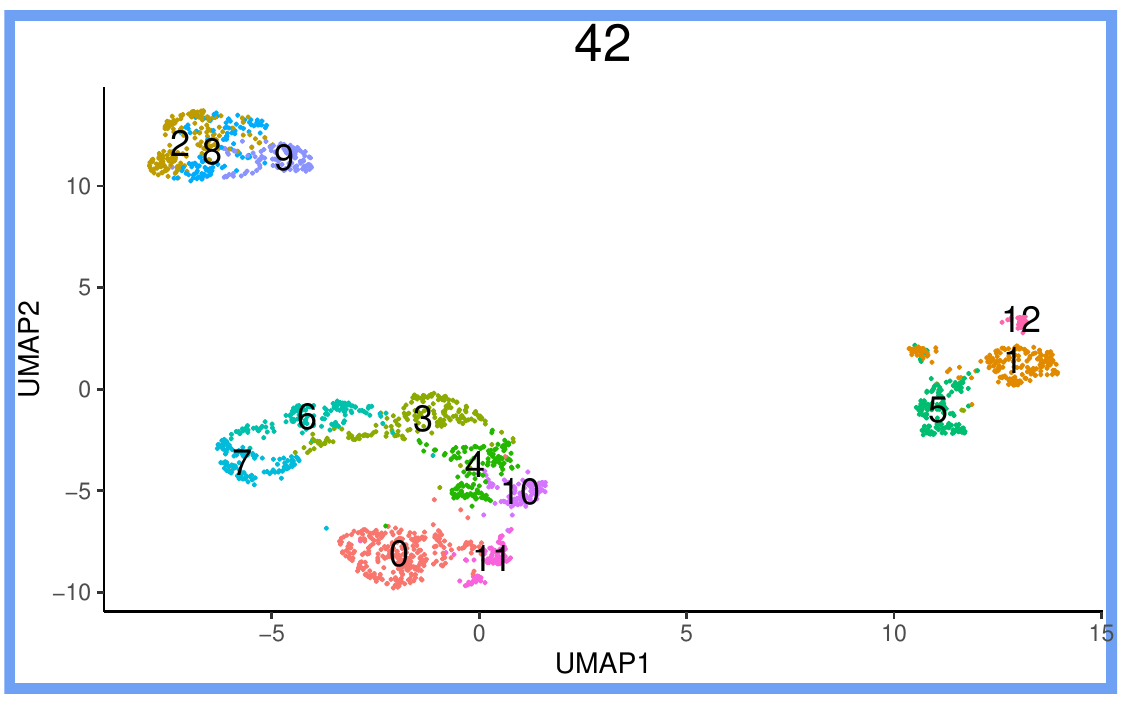
\includegraphics[width=7cm]{images/ch2/2_S1.png}
    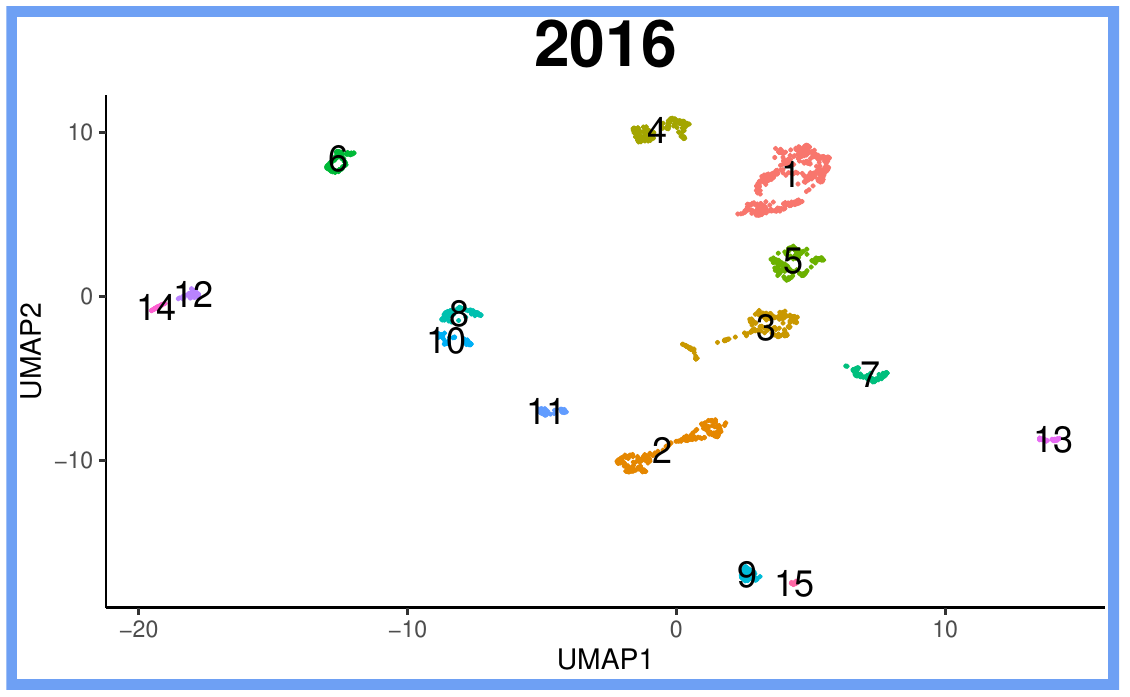
\includegraphics[width=7cm]{images/ch2/2_M1.png}
    \caption{\textbf{Partitions obtained on default values of the parameters} Clustering with Monocle (right) and Seurat (left). The title indicates the default random seed that was used.}
\end{figure}
\end{frame}

\begin{frame}{Aligning the results}
  \begin{table}[H]
    \resizebox{\textwidth}{!}{
    
            \begin{tabular}{|l|l|l|l|}
                \hline
                \textbf{Parameter name}     & \textbf{Step}                            & \textbf{Monocle value}    & \textbf{Seurat value}     \\ \hline
                \textbf{seed}               & \cellcolor[HTML]{6D9FF3}-                & 2016                      & 42                        \\ \hline
                \textbf{feature set}        & \cellcolor[HTML]{E7A101}Dim reduction    & all genes                 & HV genes                  \\ \hline
                \textbf{UMAP min dist}      & \cellcolor[HTML]{E7A101}Dim reduction    & 0.1                       & 0.3                       \\ \hline
                \textbf{UMAP n neighbours}  & \cellcolor[HTML]{E7A101}Dim reduction    & 15                        & 30                        \\ \hline
                \textbf{base embedding}     & \cellcolor[HTML]{BE809D}Graph building   & UMAP                      & PCA                       \\ \hline
                \textbf{SNN implementation} & \cellcolor[HTML]{BE809D}Graph building   & \begin{tabular}[c]{@{}l@{}}no self-neighbours\\ only direct neighbours\end{tabular} & \begin{tabular}[c]{@{}l@{}}with self-neighbours\\ direct and indirect neighbours\end{tabular} \\ \hline
                \textbf{graph type}         & \cellcolor[HTML]{BE809D}Graph building   & unweighted                & weighted                  \\ \hline
                \textbf{clustering method}  & \cellcolor[HTML]{72B980}Graph clustering & Leiden                    & Louvain                   \\ \hline
                \textbf{quality function}   & \cellcolor[HTML]{72B980}Graph clustering & CPM                       & RBConfiguration           \\ \hline
                \textbf{resolution}         & \cellcolor[HTML]{72B980}Graph clustering & 1e-4                      & 0.8                       \\ \hline
                \textbf{\#iterations}       & \cellcolor[HTML]{72B980}Graph clustering & 2                         & 10                        \\ \hline
            \end{tabular}}
            \caption{\textbf{Parameters used for aligning the results of Monocle and Seurat}}
        \end{table}
    

\end{frame}